\documentclass[11pt,
  letterpaper,
  openany,
  toc=bibliography,
  idxtotoc,
  bookmarks]{labbook}

\usepackage[utf8]{inputenc}
\usepackage[T1]{fontenc}
\usepackage[spanish]{babel}

\usepackage[margin=2.5cm]{geometry}
\usepackage{microtype}
\usepackage{graphicx}
\usepackage{amsmath,amssymb}
\usepackage{csquotes}
\usepackage{booktabs}
\usepackage{enumitem}
\usepackage{authblk}
\usepackage[spanish]{cleveref}
\usepackage[dvipsnames]{xcolor}
\usepackage{pgfplotstable}
\usepackage{siunitx}
\usepackage{subcaption}
\usepackage{multirow}

\pgfplotsset{compat=1.18}
\pgfkeys{/pgf/number format/1000 sep={\,}}

\AtBeginDocument{\decimalpoint}
\renewcommand{\arraystretch}{1.2}
\sisetup{group-digits=true,
  group-separator={\,},
  separate-uncertainty}

\usepackage[backend=biber,style=numeric]{biblatex}
\addbibresource{./references-pre-project.bib}

\usepackage{pdfbase}
\pdfinfo{
  /Title (Electron Beam)
  /Author (Sebastián Rodríguez, Laura Torres, Julián Ávila)
  /Creator (LaTeX with labbook class)
}

\title{\textbf{Rayo de Electrones} \\
Bitácora de Laboratorio}
\author{Sebastian Rodríguez \and Laura Torres \and Julian Avila}
\affil{Universidad Distrital Francisco José de Caldas}
\date{}

\begin{document}

\maketitle

\tableofcontents

\subsection{Modelo I: Campo Magnético Espacialmente Uniforme}
\label{ssec:campo_uniforme}

En una configuración de bobinas de Helmholtz, donde las corrientes fluyen
en la misma dirección, se genera un campo magnético aditivo y
notablemente uniforme en la región central entre ellas. Como primera
aproximación, se postula que el campo magnético $\boldsymbol{B}$ es
espacialmente uniforme y depende únicamente del tiempo.

El campo total es la superposición de los campos generados por cada par
de bobinas. En el formalismo de álgebra geométrica, este bivector es:
\begin{gather}
	\boldsymbol{B}(t) = B_2(t) e_{31} + B_3(t) e_{12},
	\label{eq:B_field_uniform}
	\\
	B_i(t) = \left( \frac{4}{5} \right)^{\frac{3}{2}}
	\frac{\mu_0 n I_{i}(t)}{R} =: B_0 I_i(t),
	\label{eq:B_field_magnitude}
\end{gather}
%
donde $\mu_0$ es la permeabilidad del vacío, $n$ el número de vueltas de
cada bobina, $R$ su radio, y $I_i(t)$ la corriente de alimentación. El
subíndice $i \in \{2, 3\}$ denota el eje cartesiano correspondiente.

Dada la no unicidad del potencial vectorial magnético $\boldsymbol{A}$, se
adopta el \emph{gauge simétrico}:
%
\begin{equation}
	\boldsymbol{A}(\boldsymbol{x}, t) = \frac{1}{2}
	\langle \boldsymbol{x} \boldsymbol{B}(t) \rangle_{1}.
	\label{eq:symmetric_gauge}
\end{equation}
%
Esta elección satisface correctamente la condición
$\langle \nabla \boldsymbol{A} \rangle_{2} = \boldsymbol{B}$.
El campo eléctrico inducido se deriva de
$\boldsymbol{E} = - \partial_t \boldsymbol{A}$, resultando en:
%
\begin{equation}
	\boldsymbol{E}(\boldsymbol{x}, t) = - \frac{1}{2} \langle \boldsymbol{x}
	\, \partial_t \boldsymbol{B}(t) \rangle_{1}.
	\label{eq:E_induced_uniform}
\end{equation}

\subsubsection{Análisis de la Dinámica del Campo Magnético}
\label{sssec:dinamica_b}

La estructura temporal del campo magnético, descrita en la
\cref{eq:B_field_uniform}, determina la naturaleza de la fuerza ejercida
sobre el electrón. Para visualizar esta dinámica, se analiza la
evolución del vector dual al bivector magnético,
$\boldsymbol{B}^* = \boldsymbol{B}e_{123}^{-1}$. Esto equivale a realizar
una gráfica paramétrica de la componente $B_3(t)$ en función de $B_2(t)$.

Cuando las corrientes $I_2(t)$ e $I_3(t)$ son sinusoidales, la
trayectoria resultante es una \emph{figura de Lissajous}. La morfología de
esta figura depende críticamente de la razón de frecuencias,
$\omega_2/\omega_3$, y del desfase, $\phi$, entre ambas señales.

En este experimento se utilizaron también señales cuadradas, generando
dinámicas distintas. Para dos señales cuadradas, la trayectoria traza un
perímetro rectangular, con transiciones que dependen de la relación de
frecuencias. La combinación de una señal sinusoidal y una cuadrada
produce una trayectoria confinada entre dos segmentos rectos, conectados
por arcos sinusoidales.

La \cref{fig:B_fields} ilustra estas tres configuraciones para una razón
de frecuencia de 3:1 y un desfase nulo, mostrando la rica variedad de
campos magnéticos temporales que se pueden generar.

\begin{figure}[htbp!]
	\centering
	\begin{subfigure}{0.32\linewidth}
		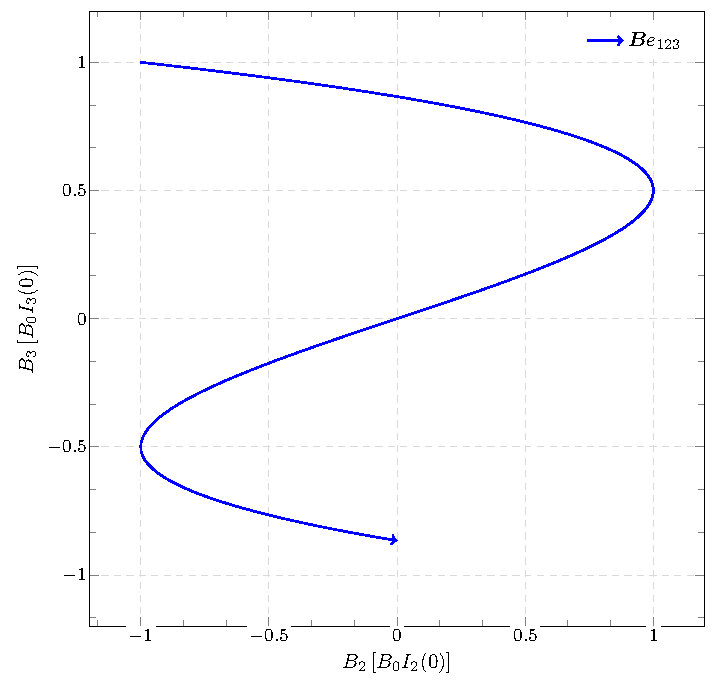
\includegraphics[width=\linewidth]{../Figures/Uniform-Field/B-sin-sin.pdf}
		\caption{Señales sinusoidales.}
		\label{fig:b_sin_sin}
	\end{subfigure}
	\hfill
	\begin{subfigure}{0.32\linewidth}
		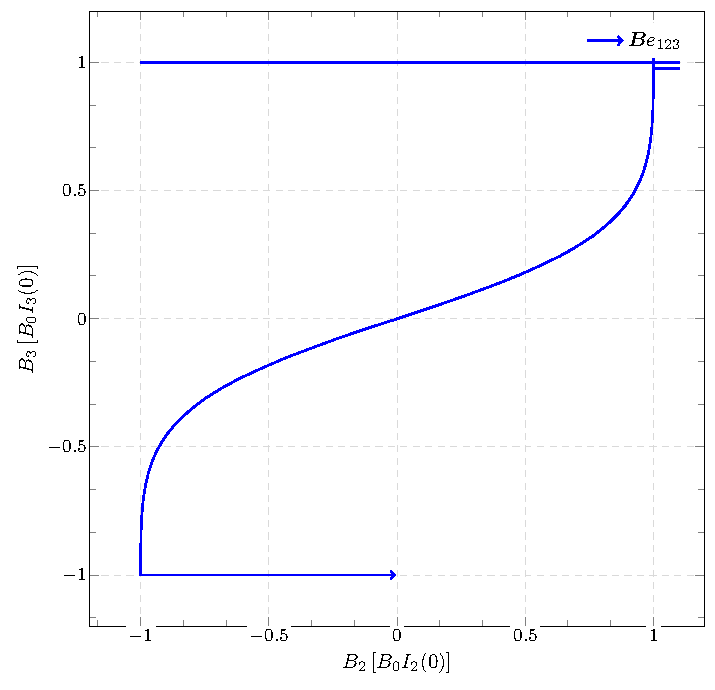
\includegraphics[width=\linewidth]{../Figures/Uniform-Field/B-square-square.pdf}
		\caption{Señales cuadradas.}
		\label{fig:b_sqr_sqr}
	\end{subfigure}
	\hfill
	\begin{subfigure}{0.32\linewidth}
		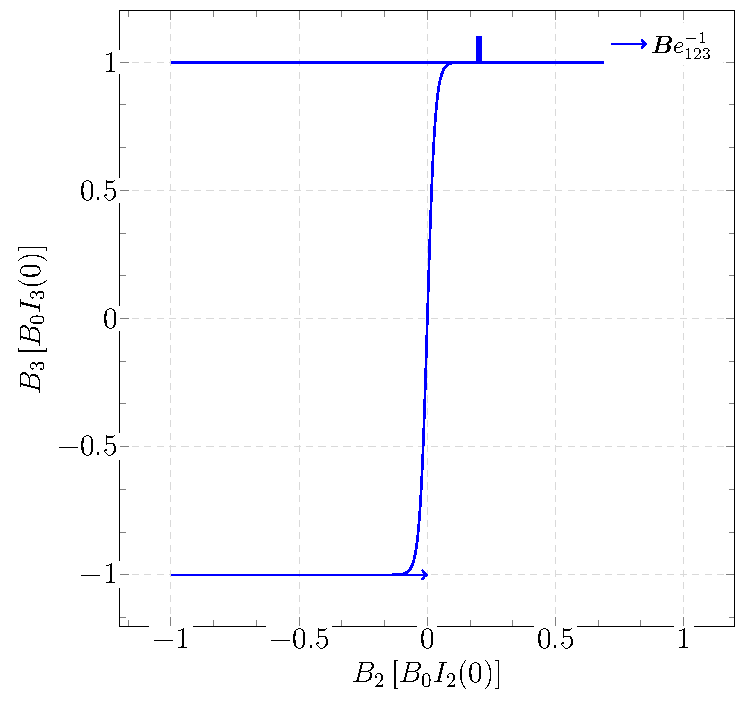
\includegraphics[width=\linewidth]{../Figures/Uniform-Field/B-sin-square.pdf}
		\caption{Señal sinusoidal y cuadrada.}
		\label{fig:b_sin_sqr}
	\end{subfigure}
	\caption{Evolución del vector de campo magnético $\boldsymbol{B}^*$ en
		el plano $yz$ para distintas formas de onda de la corriente. Se
	muestra una razón de frecuencias de 3:1 y un desfase $\phi=0$.}
	\label{fig:B_fields}
\end{figure}

\subsubsection{Análisis del Campo Eléctrico Inducido}
\label{sssec:dinamica_e}

El campo eléctrico inducido $\boldsymbol{E}$ depende de la tasa de cambio
del campo magnético, $\partial_t \boldsymbol{B}$. Su magnitud es, por
ende, proporcional a la frecuencia de las corrientes de alimentación.
A continuación, se cuantifica su efecto en comparación con el campo
magnético para las condiciones específicas del experimento.

La razón entre las magnitudes de las fuerzas eléctrica y magnética es:
%
$$
\frac{|\boldsymbol{F}_E|}{|\boldsymbol{F}_B|} \approx
\frac{|\boldsymbol{E}|}{v |\boldsymbol{B}|}
$$
%
Para una señal sinusoidal, $|\boldsymbol{E}| \approx R \omega |\boldsymbol{B}|$,
donde $R$ es el radio de las bobinas, $\omega$ la frecuencia angular y $v$
la velocidad del electrón. La razón de fuerzas es entonces $\approx R\omega/v$.

Con los parámetros del montaje, se tiene:
%
\begin{itemize}
	\item Una frecuencia $f \approx \qty{50}{\hertz}$, que implica una frecuencia
		angular $\omega = 2\pi f \approx \qty{314}{\radian\per\second}$.
	\item Una energía cinética de $\qty{4.1}{\kilo\eV}$, que corresponde a una
		velocidad del electrón de $v \approx 0.1c$.
	\item Un radio de bobinas $R$ del orden de $\qty{6.2}{\centi\meter}$.
\end{itemize}
%
Sustituyendo estos valores se obtiene:
%
$$
\frac{|\boldsymbol{F}_E|}{|\boldsymbol{F}_B|} \approx \frac{R\omega}{v}
\approx 10^{-7}
$$
%
Este resultado numérico, de orden $10^{-7}$, confirma de manera
contundente que la fuerza magnética es aproximadamente \emph{diez millones} de
veces mayor que la fuerza eléctrica. Por lo tanto, es una aproximación
justificada considerar que la dinámica es gobernada
exclusivamente por el campo magnético, omitiendo el término de
$\boldsymbol{E}$ en el modelo.


\printbibliography

\end{document}
